\begin{figure*}[t]
\caption{Network Overview}
\centering
\begin{subfigure}[b]{0.5\textwidth}
\centering
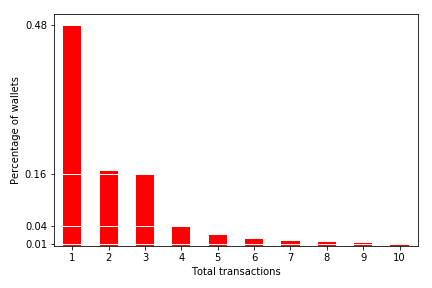
\includegraphics[height=155px]{../pics/distribution.png}
\caption{Distribution of total number of transactions}
\end{subfigure}%
\begin{subfigure}[b]{0.5\textwidth}
\centering
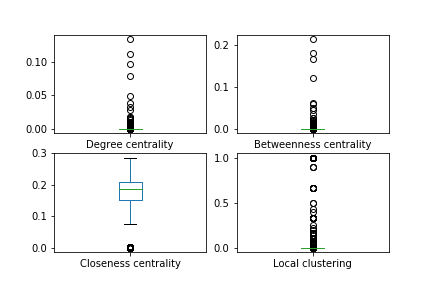
\includegraphics[height=168px]{../analysis/centrality.png}
\caption{Centrality Distribution}
\label{centralitydist}
\end{subfigure}
\end{figure*}

Looking at the rough outline of the observed period revealed that almost half of the wallets take part in one transaction during that time frame.
Roughly 16 percent of the wallets appear two or three times respectively.

Since the vast majority of accounts only seem to appear once inside the whole dataset we concluded that these are not interesting from a graph analysis perspective. 
Therefore we opted to use a subset from that data of accounts, where we could verify that they are interacting with other accounts. 
This subset consists of roughly four and a half million transactions in which 27.000 distinct wallets were either the sender or the receiver. 
From this subset we opted to create a graph in which the wallets are represented by the graph's nodes and the transactions are symbolized by the graph's edges.

Even this subset proved to be too large to handle, which means for the further graph-analysis that we were forced to rely on a random subset. 
However, if this random sample is large enough it should still give us an insight into the structure of the Ethereum network and the graph formed by this subset should still provide interpretable results.

\begin{figure*}[!ht]
\centering
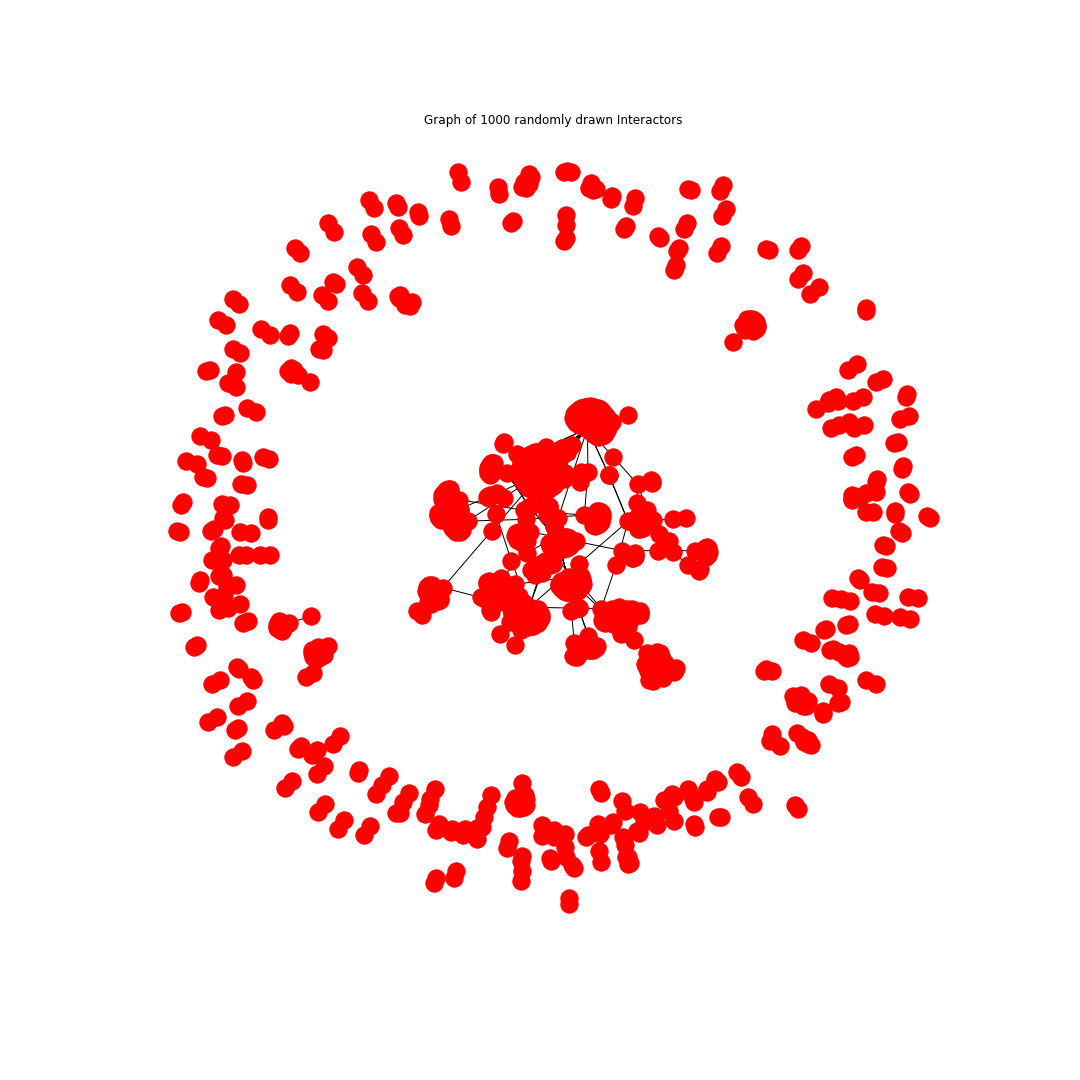
\includegraphics[scale=0.475]{../analysis/graph-subsample-1000.png}
\caption{Graph formed by a subsample of 1000 randomly drawn wallets}
\label{graphgraph}
\end{figure*}

\begin{table*}[!ht]
\centering
\caption{Centrality Distribution}
\begin{tabular}{lcccc}
\toprule
{} &  Degree centrality &  Betweenness centrality &  Closeness centrality &  Local clustering \\
\midrule
mean &             0.0001 &                  0.0001 &                0.1540 &            0.0043 \\
std  &             0.0012 &                  0.0020 &                0.0782 &            0.0636 \\
min  &             0.0000 &                  0.0000 &                0.0000 &            0.0000 \\
25\%  &             0.0000 &                  0.0000 &                0.1522 &            0.0000 \\
50\%  &             0.0000 &                  0.0000 &                0.1876 &            0.0000 \\
75\%  &             0.0000 &                  0.0000 &                0.2072 &            0.0000 \\
max  &             0.1344 &                  0.2149 &                0.2862 &            1.0000 \\
\bottomrule
\end{tabular}

\label{graphtable}
\end{table*}

\begin{figure*}[!ht]
\centering
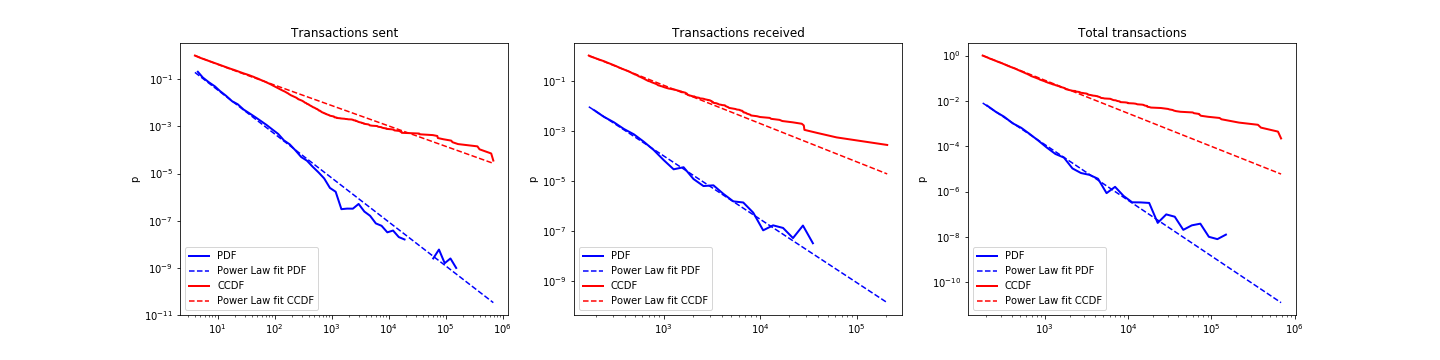
\includegraphics[width=\textwidth]{../analysis/power-law-fit.png}
\caption{Comparison with random graphs}
\label{powerlaw}
\end{figure*}


Figure \ref{graphgraph} displays the graph built from a random subsample of 1000 transactions, where again the nodes represent the different wallets and the edges stand for an observed transaction between them. 
The size of the node stands for the transaction's value. We can clearly see that most of the accounts form connections that consist of only two wallets and it is highly likely that these are also the accounts which are only observed once in the entire dataset. 

Even here it is possible to see that there are subclusters of highly connected nodes associated with a high transaction value located in the middle of the graph. 
This appears despite the small sample size, which has to mean that these nodes in the center of the graph are important actors inside the network whose position will most likely become more pronounced the larger we choose the sample size to be. 
From this first glimpse{\parfillskip0pt\par}

\noindent at the network we would expect to find two tendencies inside the dataset. 
First, we expect a large number of nodes which are associated with low centrality measures and clustering coefficients. 
Secondly we expect to find some collections of nodes that form subgroups and within these subgroups we should be able to locate some nodes that play a tangible role in their respective local neighborhoods. Both of those observations do fit into the notion of a random graph, where we would expect a large number of loosely connected nodes with a low degree and an exponentially lower quanity of nodes which have a higher degree and who play a more central role inside the network.

Note nonetheless, that figure \ref{graphgraph} provides only a rough outline since it is only using one thousand out of the 7.3 million available transactions. 
We pick a comparatively small sample size for this graph in order to avoid overplotting, the further analysis however uses a larger subsample of 100000 transactions.

The results of the larger subsample are summarized in table \ref{graphtable} and figure \ref{centralitydist}. 
For the Degree Centrality we can observe a highly skewed distribution, where the mean lies at $\bar{C_D} = 0.0001$, whereas the first three quartiles remain firmely at $0$. 
This indeed confirmes our previous suspicion that most nodes inside this network are merely loosely connected, even after removing the most isolated and remote nodes of the initial dataset. 
This means that most wallets interact only with are very limited set of other wallets and that it is highly uncommon for a node to accept transactions from many different wallets.

When looking at the results for the graph's Betweenness-Centrality, we can see a similiar pattern. 
The mean lies at $\bar{C_B}=0.0001$ and all three quartiles are, again, $0$. This means that the Betweenness centrality's distribution is also heavily skewed, which indicates that only a few nodes act as a mediator for their neighbors. 
This should not come as a surprise, since most of the nodes have a very low degree to begin with.

The Closeness centrality between all nodes paints a different picture. Its distribution is still skewed, however it is not as extremely skewed as the measures that have been discussed so far. 
The mean lies at $\bar{C_C}=0.15$ with a standard deviation of $s_{C_C} = 0.078$. 
Note that this measure needs to be interpreted with care. 
Most of the nodes are disconnected, and thus do not have a connecting path at all. 
If a node $j$ cannot be reached from a different node $k$ there exist two common propositions in the literature. 
Either $d(j, k) = 0$ or $d(j, k)=\infty$. 
Most implementations rely on the former convention rather than the latter, since it avoids values that cannot interpreted as a number. This is also the convention that is implemented in the \texttt{networkx} module for the \texttt{Python} programming language \cite{networkx}. But this also means that the closeness centrality should be interpreted as a local measure since the distances in the normalizing factor in (\ref{closeness}), which are calculated as $$\sum\limits_{i=1}^g d(n, i),$$ will contain numerous zero-valued summands. So actually, this measure only makes sense for nodes that are of a degree $k$ that is larger than three, since nodes of a lesser degree are necessarily close to each other.

The Local clustering coefficient accross the nodes is again highly skewed to the left. The mean lies at $\bar{C_L}=0.004$ at a standard deviation of $s_{C_L}=0.063$. Again the quartiles are all planted at $0$. Note however, that there exist some nodes whose Local clustering coefficient reaches as far as $C_L(n)=1$. This means that there are some nodes who are fully connected within their local cluster, which means that all triangles within that clique are centered around that node $n$. This, in turn, means that there are some nodes which are perfectly connected inside their neighborhood.

So far all these findings indicate that the model of a random graph would be a good approximation of the real world data. In order to test this assumption in a graphical manner, we would like to compare the empirical density functions of the degrees against the theoretical powerlaw distribution. Remember that, in a random graph, the random variable $K(n)$ that describes the degree of a node $n$ follows a powerlaw distribution $$P(K(n)=k)\propto k^{-\alpha},$$ where $\alpha$ is some constant that has to be determined by Maximum-Likelihood methods \cite{graphintro}. Figure \ref{powerlaw} presents the results for the empirical probability density function (PDF) and the complementary cumulative distribution function (CCDF). The CCDF is primarily used in the domain of signal processing and measures the the amount of time a signal spends above the mean power level of the measured signal. Equivalently, it assesses the probability that the signal power will be above the average power level \cite{ccdf2015}.

In order to reflect the difference in the roles accross the network such as the reciever or the sender of a transaction, we split the analysis into three different parts. First, we look at the distribution of the directed graph that is focusing on the actors that iniatate a transactions, i.e. the senders. Second, we look at the network formed by the receivers of a transaction and finally we look at the whole undirected graph that contains both receivers and senders. The results are displayed in figure \ref{powerlaw}. The PDF is shown by the blue line and the CCDF is represented by the red line. A high overlap between the dashed and the solid line indicates a good fit of the empirical distribution compared to the theoretical. Thus the probability density function of a perfectly random network would lie on its respective dashed line.

In the leftmost part of figure \ref{powerlaw} we can see for the senders that the tails of the empirical PDF are closely following the theoretical distribution of the random graph. However, in the central part we observe one large deviation from the distribution of a random network. In particular, this means that - under a random graph - we would have expected more nodes that have a middling degree, i.e. $k=3$, $k=4$, and so forth. Instead, we observe a large number of loosely connected nodes.

The same holds for the sender's CCDF. The lower tail of the distribution follows the random graph closely, whereas the central part is too low, and the upper tail is too high for a random graph.

Looking at the wallets at the receiving end of a transaction, in the middle part of figure \ref{powerlaw}, we can discern a similar pattern. Both, the line for the PDF, as well as the line for the CCDF begin by closely following the theoretical distribution and begin to deviate after passing the median. Again we observe a density at the lower tail that is very similar to what we would expect from a random graph.

However, the most clear indicator of that pattern is shown for the composite graph, that contains both senders and receivers, in the rightmost part of figure \ref{powerlaw}. Here we observe a very pronounced deviation from the course of both the theoretical PDF and CCDF after reaching the median. Again, this is a clear indicator that there are too many nodes with a comparatively high degree, for this to be a random network.

